\hypertarget{genesting_8c}{
\section{Referencia del Archivo genesting.c}
\label{genesting_8c}\index{genesting.c@{genesting.c}}
}


\subsection{Descripci\'{o}n detallada}
Aqui estan las estructuras principales del programa la estructura es muy sencilla 

Definici\'{o}n en el archivo \hyperlink{genesting_8c-source}{genesting.c}.

{\tt \#include $<$stdio.h$>$}\par
{\tt \#include $<$stdlib.h$>$}\par
{\tt \#include $<$math.h$>$}\par
{\tt \#include \char`\"{}genesting.h\char`\"{}}\par
{\tt \#include \char`\"{}polygon.h\char`\"{}}\par
{\tt \#include \char`\"{}polygon\_\-holes.h\char`\"{}}\par


Dependencia gr\'{a}fica adjunta para genesting.c:\begin{figure}[H]
\begin{center}
\leavevmode
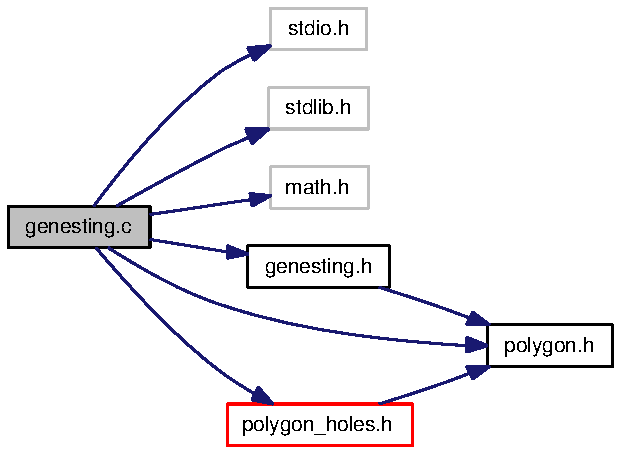
\includegraphics[width=167pt]{genesting_8c__incl}
\end{center}
\end{figure}
\subsection*{Funciones}
\begin{CompactItemize}
\item 
\hyperlink{struct__genesting}{genesting} $\ast$ \hyperlink{group__genetic_g6fed4910dd1f6172bb5a4e35a97bbe56_g6fed4910dd1f6172bb5a4e35a97bbe56}{leer\_\-archivo} (char $\ast$arc\_\-name)
\item 
void \hyperlink{group__genetic_g1daa6a4e8af34b8b16a48fc2f3701f1c_g1daa6a4e8af34b8b16a48fc2f3701f1c}{genesting\_\-init} (\hyperlink{struct__genesting}{genesting} $\ast$g)
\item 
void \hyperlink{group__genetic_g3f63f4034274d731cb3fdf3200c64d41_g3f63f4034274d731cb3fdf3200c64d41}{genesting\_\-show} (\hyperlink{struct__genesting}{genesting} $\ast$g)
\end{CompactItemize}
